\chapter{Développement d'une méthode d'angiographie dynamique avec deux angles d'or.}

\section{Contexte}

Ces dernières années, le développement de nombreux modèles murins mimant des pathologies s'est fortement développé dans le domaine de la biologie vasculaire. Pour caractériser ces modèles mais aussi pour pouvoir tester des thérapies, il est nécessaire de visualiser des changements physiopathologiques ou anatomiques de manière longitudinale et non-invasive. 
L'angiographie par résonance magnétique de type temps-de-vol (TOF) est une méthode de choix pour étudier les pathologies vasculaires. En effet, c'est une technique ayant un contraste vasculaire endogène lié à l'entrée de sang non saturé dans le volume d'imagerie et donc ne nécessitant pas d'injection d'agent de contraste. De plus c'est une méthode d'imagerie rapide permettant d'obtenir des images en trois dimensions avec des temps d'acquisitions raisonnables et donc :
\begin{enumerate}
\item D'obtenir un meilleur signal sur bruit (SNR)
\item D'augmenter la résolution spatiale dans la direction de coupe
\item De réduire le temps d'écho des séquences
\end{enumerate}
Effectuer l'imagerie vasculaire en 3D est donc très intéressant car cella permet d'atteindre de forte résolution qui sont nécessaire pour visualiser des vaisseaux ayant des diamètres inférieurs à 200 $\mu$m chez la souris ainsi que de limiter les artéfacts de flux sanguin grâce à des temps d'échos plus court (Voir section \ref{subsec:MouvEtFlux}).

Cependant, l'imagerie TOF ne permet d'obtenir que des informations anatomiques et dans certains cas, il peut être intéressant d'étudier la dynamique des flux sanguins. En effet il a été montré que la vitesse du flux sanguin est un paramètre important qui permet de dépister certaines anomalies du système circulatoire sanguin. Par example, un flux sanguin important dans le polygone de Willis peut être le signe d'une sténose d'une artère en amont \cite{Essig:1996ve}. Ou bien, une diminution du flux dans les artères carotides peut prédire l'apparition d'un accident vasculaire cérébral ischémique \cite{Bai2007Lower-blood-flo}. Accéder à cette information chez le petit animal est donc essentiel dans le cadre d'une étude sur une large cohorte d'animaux pour en limiter la variabilité dans de nombreux modèles de pathologies comme l'hypertension pulmonaire \cite{Cochet:2013dk}, l'artérioschérose \cite{La-Roque:2011rw} et pour caractériser leurs réponses à un traitement.

Chez l'humain la méthode ARM de mesure de vitesse des flux la plus utilisé est l'imagerie de contraste de phase \cite{Petersson:2015aa}. Celle-ci permet de calculer la vitesse des spins dans chaque voxel grâce l'ajout d'un gradient bipolaire. Toutefois, cette méthode est difficilement applicable chez le petit animal en 3D pour deux raisons. D'une part, cette méthode requiert d'encoder la vitesse selon les 3 directions ce qui nécessite de répéter l'expérience au moins 4 fois. Surtout, la précision de la mesure est inversement proportionnelle au signal dans l'image ce qui handicapent les méthodes 3D qui saturent le signal sanguin en excitant à chaque répétition tout le volume. C'est pourquoi ces méthodes sont donc principalement appliquées chez le petit animal en 2D. 

Il existe une autre méthode d'ARM permettant de visualiser la dynamique des flux qui a été développé précédemment au sein du laboratoire sur des modèles murins \cite{Miraux:2006fu}. Celle-ci consiste, après la détection d'un pic ECG, à saturer le signal dans le volume puis à recueillir le signal du sang frais progressant dans les vaisseaux. L'utilisation d'un module de saturation d'une faible durée avant le recueil des signaux avec une séquence d'écho de gradient rapide standard permet d'obtenir une résolution temporelle des images égale au TR d'une séquence écho de gradient classique. Malgré les difficultés liées aux paramètres physiologiques de la souris (rythme cardiaque élevé et volume sanguin faible), la méthode a permis la mesure du flux sanguin dans diverses artères: carotides \cite{Miraux:2006fu}, pulmonaires \cite{Cochet:2013dk} et même coronaires \cite{Cochet:2010ec}. Malgré tout, cette méthode peut encore être améliorée que ce soit au niveau du temps totale de l'expérience, de la résolution temporelle ou du signal obtenue.
%\begin{figure}[H]
%\centering
%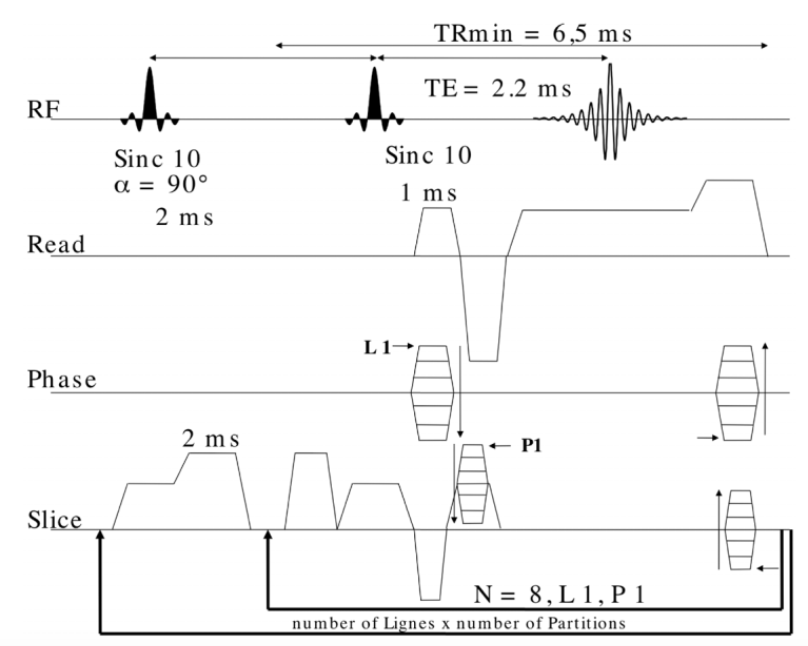
\includegraphics[scale=0.5]{./figure/chap3/SeqSylvain.png}
%\caption[Séquence ARM Sylvain et al.]{\label{fig:SeqSylvain} Chronogramme de la séquence utilisé pour obtenir une ARM sang-blanc résolue dans le temps. L = Nombre de ligne, P = Nombre de partition, N = Nombre d'images résolues dans le temps reconstruites. (Figure extraite de Sylvain et al. 2006)}
%\line(1,0){400} \\ \end{figure}


L'idée que je développerai dans ce chapitre est de combiner la méthode d'angiographie dynamique par temps-de-vol avec des trajectoires 3D radiales plutôt que cartésiennes. Car, comme mentionné dans le chapitre précédent, l'imagerie radiale peut fournir des images de bonne qualité avec un facteur de sous-échantillonnage important. De plus, nous avons implémenté une méthode de répartition pseudo-aléatoire nous permettant d'obtenir une certaines flexibilité durant la reconstruction pour adapter la résolution temporelle selon la qualité des images désirées.

\section{Flexibilité dans les trajectoires radiales}

L'un des inconvénient de la trajectoire cartésienne est son manque de flexibilité dans la reconstruction de l'image. Une fois que la résolution temporelle a été déterminé par le nombre de ligne successives à recueillir pour chaque répétition, il est difficile d'obtenir des images de bonne qualité (à partir du même jeu de donnée) avec une résolution temporelle différente.
Les trajectoires radiales sont plus flexibles car elles permettent de reconstruire des images intermédiaires sans attendre d'avoir recueillis toutes les projections de l'espace de Fourier. Mais, comme montré dans la figure \ref{fig:SousEchant}, cela est très dépendant de la méthode de répartition des projections employées.
\begin{figure}[H]
\centering
\line(1,0){400} \\
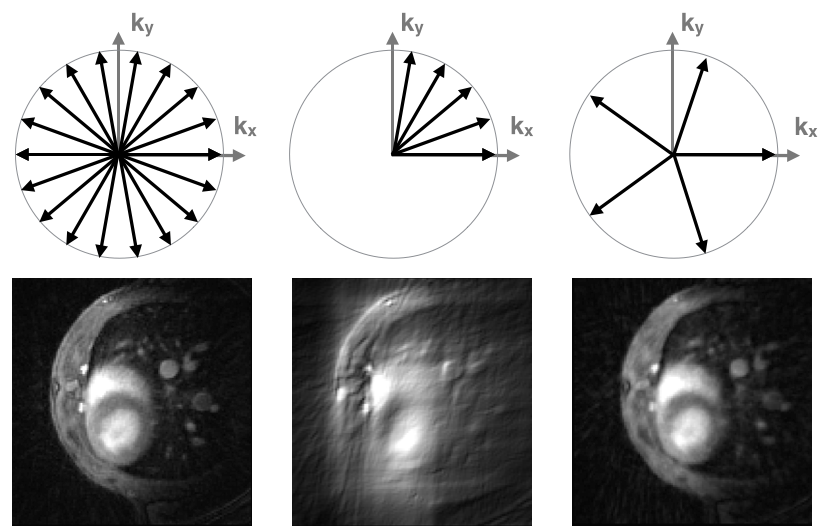
\includegraphics[scale=0.5]{./figure/chap3/SousEchan.png}
\caption[Sous-échantillonnage]{\label{fig:SousEchan} Vue axiale obtenue avec une séquence UTE 2D sur le coeur de souris. A gauche : l'image est reconstruite avec les 402 projections pour atteindre le critère de nyquist. Au centre : l'image est acquises avec 100 projections réparties de manières adjacentes par rapport au cas idéal à gauche. A droite : l'image est reconstruite avec 100 projections réparties de manière uniforme sur le plan.}
\line(1,0){400} \\ \end{figure}
De nombreuses méthodes de répartition différentes des projections 2D et 3D ont été étudiées. Winkelmann et al. \cite{Winkelmann:2007fk} et Song et al. \cite{Song:2000fk} ont montré que l'imagerie radiale 2D est plus flexible en utilisant un angle d'or, dérivé du facteur d'or (décris dans la prochaine section). Par example en imagerie de prise de contraste dynamique, en positionnant les projections dans l'espace de Fourier avec cet angle, il est possible à partir de n'importe quelle position de reconstruire une image. Le nombre de projection a utiliser peut-être adapté pour modifier à la résolution spatiotemporelle. Chan et al. \cite{Chan:2009uq} ont montré qu'il était possible d'étendre la notion d'angle d'or à l'imagerie radiale 3D et ont montré son application à l'imagerie dynamique de prise de contraste dans les tumeurs du sein.

Pour notre projet d'imagerie dynamique TOF, la méthode d'acquisition est différentes puisque nous utiliserons des projections recueillies à une certaines positions après la saturation du signal. Le travail de répartition pseudo-aléatoire doit donc se faire selon ces projections. 
L'utilisation d'une méthode de répartition des projections aléatoire aura donc aussi un gain différent : Il nous sera possible d'arrêter la séquence avant la fin de l'acquisition et tout de même obtenir une image de bonne qualité. Mais surtout en cas de projections corrompues, par example par le mouvement respiratoire ou bien par des arythmies cardiaques qui modifieront la vitesse mesurée du flux, Il sera possible lors de la reconstruction de les retirer sans que cela ne crée de zone étendue sans information dans l'espace de Fourier.

\subsection{Angle d'or}

\subsubsection{Facteur d'or 1D et angle d'or 2D}

Le facteur d'or, hormis ces aspects "esthétiques" dans la nature, a des propriétés mathématiques intéressantes. En effet, le facteur d'or est fortement lié à la suite de Fibonacci. Dans cette suite, chaque term est la somme des deux précédents :
\begin{equation}
F_n=\{0,1,1,2,3,5,8,13...\}\ \ where\ F_n=F_{n-1}+F_{n-2}
\end{equation}
Lorsque la limite des termes approches l'infini, le ratio des deux termes successifs de cette suite approche le facteur d'or $\phi$:
\begin{equation}
\lim_{n \to \infty}\frac{F_n}{F_{n+1}}=\phi=\frac{\sqrt{5}-1}{2}
\end{equation}
Géométriquement, le facteur d'or peut être décrit comme une méthode permettant de découper un segment de longueur unitaire. Ce partitionnement est effectué de manière à ce que le rapport de 1 sur x soit le même que le rapport de x par rapport à tout le segment:
\begin{equation}
\frac{1}{x}=\frac{x}{x+1}
\end{equation}
Cette équation quadratique $x^2=x+1$ a pour solutions les racines $(1+\sqrt{5})/2 \simeq 1,618$ et $(1-\sqrt{5})/2 \simeq -0,618$. La racine la plus grande est définie comme le facteur d'or $\Phi \simeq 1;618$ et la plus petit comme le conjugé du facteur d'or $\phi=1/\Phi\simeq0,618$.
La figure \ref{fig:1dGold} montre le placement des points des points sur un segment unitaire au cours du temps. Le premier point est positionné exactement à la valeur du facteur d'or 0,61893. Le positionnement des 5 premiers points ainsi que répartition des 30 points illustrent comment le facteur d'or peut être utilisé pour bien répartir spatialement et temporellement des points en particulier par rapport à la distribution des 30 points positionnés aléatoirement qui donne des espaces vides plus important.
Pour passer du facteur à l'angle d'or, il suffit de multiplier la valeur $\{m\phi\}$ par $360\degres$
\begin{figure}[H]
\centering \line(1,0){400} \\

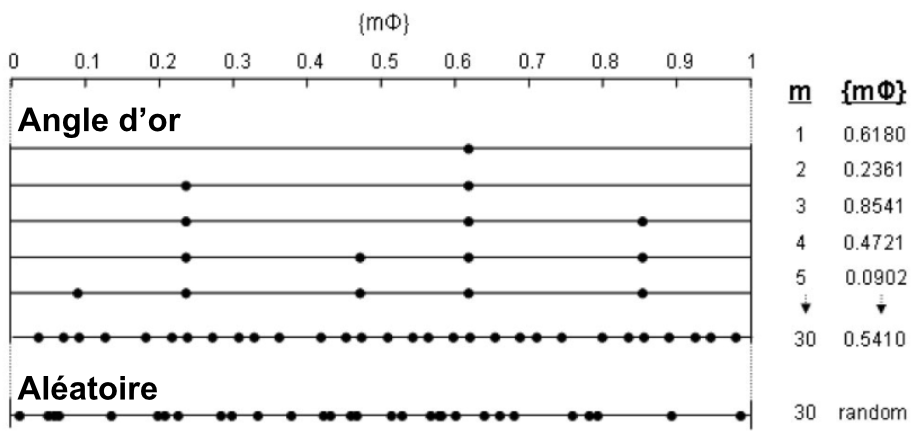
\includegraphics[scale=0.5]{./figure/chap3/1dGold.png}
\caption[Répartition 1D]{\label{fig:1dGold} Les points sont réparties sur un segment unitaire avec un intervalle régulier correspondant au modulo de $\{m\phi\}$ ou m est un entier. La distribution avec le facteur d'or est montré pour une valeur de m de 1 à 5 ainsi que pour une valeur de 30. Une répartition aléatoire de 30 points est donnée à titre de comparaison.}

\line(1,0){400} \\ \end{figure}

\subsubsection{Facteur d'or 2D}

Pour obtenir une méthode d'angle d'or 3D, il est nécessaire de définir les valeurs multidimensionnelles de facteur d'or. Pour cela, nous devons définir le facteur d'or selon une nouvelle approche :  Nous pouvons exprimer le facteur d'or 1D grâce à une suite de vecteur 2 $\times$ 1 :
\begin{equation}
u_1=[F_0,F_1]=[0,1],\ 
u_2=[F_1,F_2]=[1,1],\ 
u_3=[F_2,F_3]=[1,2],\ 
u_4=[F_3,F_4]=[2,3] \ ...
\end{equation}
Chaque  valeur $u_i$ peut aussi être déterminé à partir de $u_{i-1}$ en utilisant une transformation de Fibonacci $M_{Fib}$ à $u_{i-1}$ :
\begin{equation}
u_i=M_{Fib} \cdot u_{i-1}\Rightarrow 
\left(
\begin{array}{c}
F_{i-1} \\
F_{i}
\end{array}
\right)=\left(
\begin{array}{c c}
0 & 1 \\
1 & 1
\end{array}
\right)\left(
\begin{array}{c}
F_{i-2} \\
F_{i-1}
\end{array}
\right)
\end{equation}
Si $M_{Fib}$ est appliqué de manière récursive pour obtenir les vecteurs en tendant vers l'infini, le rapport des élements de ce vecteur converge vers le facteur d'or. L'écriture sous forme matricielle permet de trouver le facteur d'or à partir de la suite de Fibonacci en utilisant ces valeurs propres. Le facteur d'or peut être obtenu à partir du vecteur propre $v$ déterminé à partir de : $M_{Fib} v=\lambda v$ (où $\lambda$	est la valeur propre). Si le vecteur propre $v=[v_1,v_2]$ est écris de manière à ce que $v_2=1$, $v_1$ devient le facteur d'or. Pour trouver $v$ il faut calculer $det(\lambda I-M_{Fib})=0$ ce qui donne l'équation caractéristique ($\lambda ^2 = \lambda +1$) que nous avons vu dans la partie précédente et dont les racines nous donnent le facteur d'or 1D.

L'avantage avec l'approche utilisant les valeurs propres est que l'on peut facilement l'étendre pour obtenir les facteurs d'or multidimensionnels pour l'imagerie radiale 3D. La suite de Fibonacci est alors modifiée de cette manière :
\begin{equation}
G_i=G_{i-1}+G_{i-3} \ with \ initial \ conditions \ G_0=0,\ G_1=1,\ G_2=2
\end{equation}
La suite de Fibonacci peut aussi être écrite de manière récursive, où $M_{Fib}$, est maintenant la version modifiée de la transformée de Fibonacci.
\begin{equation}
u_i=M_{Fib} \cdot u_{i-1}\Rightarrow 
\left(
\begin{array}{c}
G_{i-2} \\
G_{i-1} \\
G_{i}
\end{array}
\right)=\left(
\begin{array}{c c c}
0 & 1 & 0 \\
0 & 0 & 1 \\
1 & 0 & 1
\end{array}
\right)\left(
\begin{array}{c}
G_{i-3} \\
G_{i-2} \\
G_{i-1}
\end{array}
\right)
\end{equation}
Cette matrice a pour valeur propre réelle $\lambda=1.4656$ et le vecteur propre $v=[0.4656, 0.6823, 1]$. Ce qui donne des valeurs pour les facteurs d'or 2D : $\phi_1=v_1=0.4656$ et $\phi_2=v_2=0.6823$.

Les facteurs d'or 2D sont une base pour générer spatialement et temporellement une bonne distribution des points dans un carré unitaire (figutr \ref{fig:2DGold}.a) pour lequel les coordonnées des points sont définies par $(x,y)=({m\phi_1},{m\phi_2})$ pour m = 1,2,3, ... Une distribution aléatoire a été généré pour comparaison dans la figure \ref{fig:2DGold}.b. avec les coordonnées $(x,y)=(r_1,r_2)$ où $r_1$ et $r_2$ sont des variables aléatoires qui ont les même probabilités d'apparaitre entre 0 et 1.
\begin{figure}[H]
\centering \line(1,0){400} \\
\includegraphics[scale=0.4]{./figure/chap3/2DGoldCarre.png}
\caption[Répartition 2D]{\label{fig:2DGold} Distribution de points sur un carré unitaire généré par le facteur d'or 2D (a) et une distribution aléatoire (b).}
\line(1,0){400} \\ \end{figure}

\subsubsection{Angle d'or 3D}

L'implantation de l'angle 3D nécessite une modification topologique du cube unitaire vers la surface d'une sphère unitaire. La figure \ref{fig:GoldDz} montre une vue de côté d'un espace de Fourier hémisphérique ayant un rayon unitaire ($R = 1$). Si nous découpons l'hémisphère selon des plans orthogonaux à $k_z$, l'aire de la surface de n'importe laquelle de ces zones ne dépend seulement que de l'épaisseur dz. En effet, l'aire de la surface obtenue à partir d'une valeur dz infinitésimale à la hauteur h est égale à $dA = 2\pi \cos(\beta)ds$. Géométriquement, on peut montrer que $ds = dz/\cos(\beta)$, l'aire de la surface est donc égale à $dA = 2\pi dz$, qui est indépendante de la hauteur h. C'est pour cela que positionner des points équidistants selon l'axe $k_z$ donne une distribution uniforme de point sur la sphère.
\begin{figure}[H]
\centering \line(1,0){400} \\
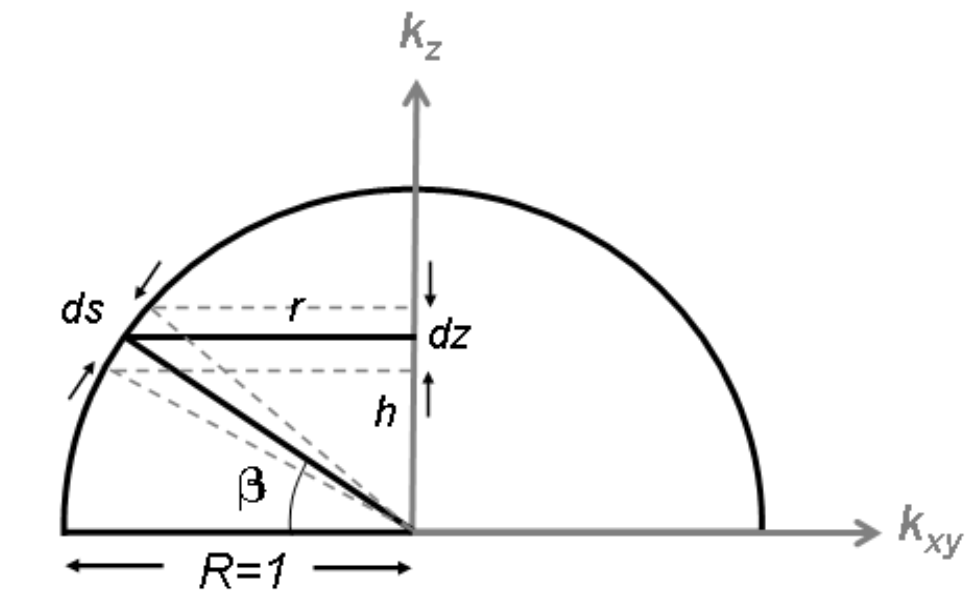
\includegraphics[scale=0.3]{./figure/chap3/GoldDz.png}
\caption[Transformation topologique]{\label{fig:GoldDz} L'aire de la surface latérale d'une sphère est proportionnel à dz et indépendante de la hauteur h de la zone.}
\line(1,0){400} \\ \end{figure}

Ici, nous utilisons une méthode de répartition des projections pour l'imagerie 3D qui utilisent $\phi_1$ pour déterminer la position selon l'axe $k_z$ et $\phi_2$ pour déterminer l'angle polaire de la projection dans le plan $k_x-k_y$ (figure \ref{fig:Gold3D}) selon les équations suivantes :
\begin{equation}
\begin{array}{c}
\Phi_i=2\pi \times mod(\phi_1 \times i,1) \\
\theta_i=acos(mod(\phi_2 \times i,1))
\end{array}
\end{equation}
où i est le numéro de la projection. Cette implémentation de l'angle d'or 3D ne fonctionne que pour l'imagerie projection-reconstruction car avec une trajectoire UTE un des hémisphères ne sera jamais échantillonné. Pour la trajectoire angle d'or 3D UTE, il faut modifier le calcul de $\theta$ :
\begin{equation}
\theta_i=2 \times acos(mod(\phi_2 \times i,1))-1
\end{equation}

\begin{figure}[H]
\centering \line(1,0){400} \\
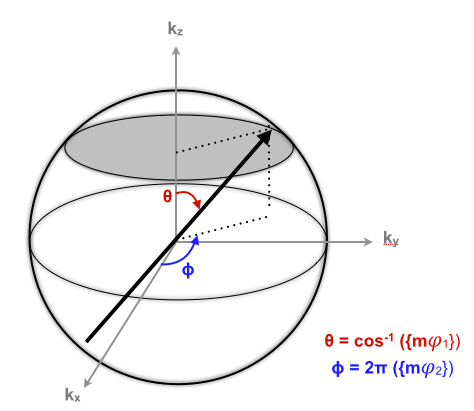
\includegraphics[scale=0.4]{./figure/chap3/Gold3D.png}
\caption[Angle d'or 3D]{\label{fig:Gold3D} Positionnement des projections radiales dans l'espace de Fourier basé sur l'angle d'or 3D.}
\line(1,0){400} \\ \end{figure}

\subsection{Flexibilité dans les séquences résolues dans le temps.}

\subsubsection{Séquence résolue dans le temps ou ciné}
\begin{figure}[H]
\centering \line(1,0){400} \\
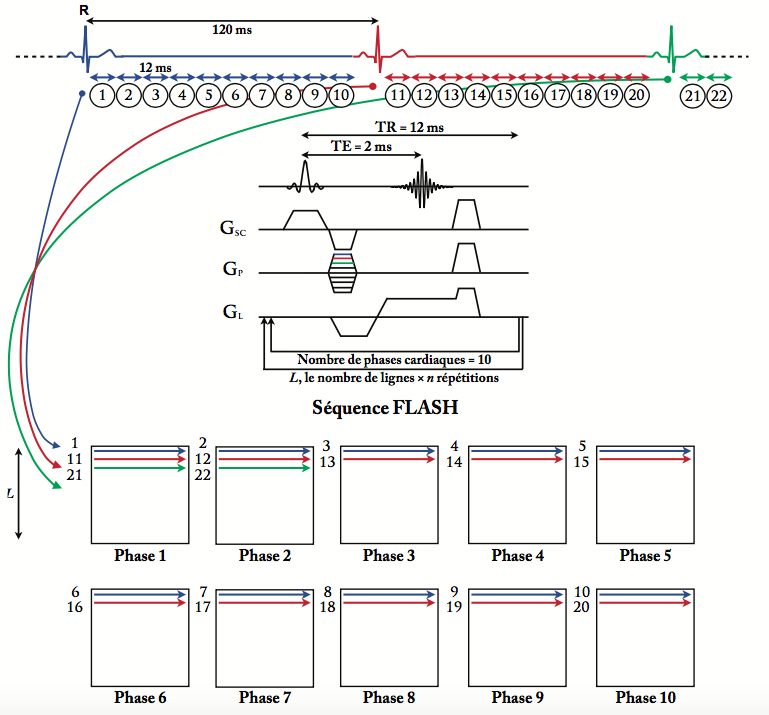
\includegraphics[scale=0.4]{./figure/chap3/SeqProspective.png}
\caption[Sequence prospective]{\label{fig:SeqProspective} Synchronisation cardiaque prospective de l'acquisition IRM sur le rythme de l'ECG. Ici, l'intervalle de temps entre 2 ondes R de l'ECG est de 120 ms chez la souris anesthésiée. Le TR de la séquence utilisée étant de 10 ms, il est possible d'imager 10 phases du cycle cardiaque. La déction d'une onde R de l'ECG déclenche la lecture de la même ligne 10 fois de suite, pour les 10 espaces de fFourier, correspondant aux 10 phases. La détection de l'onde R suivante entraîne la lecture de la ligne suivante pour chacune des 10 phases et ainsi de suite jusqu'au remplissage des L lignes de chacun des 10 espaces de Fourier. (Lefrançois, 2011)}
\line(1,0){400} \\ \end{figure}

Généralement en imagerie résolue dans le temps, N signaux IRM sont recueillies successivement avec la même trajectoire dans l'espace de Fourier. Cela est répété de manière à pouvoir remplir N espaces de Fourier complets afin de pouvoir reconstruire N images (souvent appelé image ciné) comme expliqué dans la figure \ref{fig:SeqProspective}. 
Lorsque les temps de répétition sont courts par rapport aux mouvements dynamiques que l'on souhaite observer la différence entre les images est très faible et l'on obtient donc une redondance importante dans les informations contenues dans l'espace de Fourier comme illustré dans la figure \ref{fig:DiffDynamique}. Or, comme expliqué dans la section \ref{subsec:KSpaceRegion}, il est possible d'exploiter seulement hautes fréquences pour augmenter la résolution de l'image.
Cependant la méthode standard d'imagerie résolue dans le temps ne permet pas de flexibilité spatiotemporelle entre les différentes images reconstruites. Ce constat a lieu que l'on utilise des trajectoires cartésiennes ou non-cartésiennes car elle provient seulement du fait que les trajectoires utilisés entre les images cinés soient les mêmes. Pour résoudre cela, il est donc nécessaire de modifier les trajectoires entre les cinés de manière à pouvoir ensuite les manipuler par example en additionnant deux espaces de Fourier pour gagner en résolution spatiale et signal mais perdre en résolution temporelle. 
\begin{figure}[H]
\centering \line(1,0){400} \\

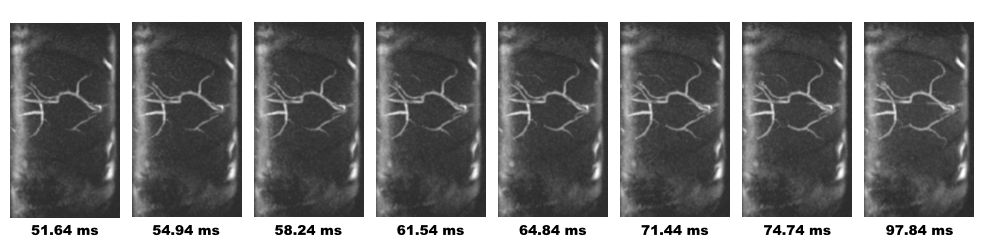
\includegraphics[scale=0.5]{./figure/chap3/DiffDynamique.png}
\caption[Différence entre des images de flux dynamique]{\label{fig:DiffDynamique}Images de projection d'intensité maximum (MIP) coronales d'un cerveaux de souris obtenues avec une séquence angiographie résolue dans le temps. Les images sont acquises consécutivement avec une séquence ayant un $TR = 3,3 ms$.}

\line(1,0){400} \\ \end{figure}

\subsubsection{Angle d'or ciné}

La méthode vers laquelle nous nous sommes dirigés a été de recueillir le signal de chaque cycle cardiaque avec des trajectoires similaire mais subissant seulement une rotation autour de l'axe $k_z$. L'angle que nous avons décidé d'employer $\Phi d_j$ est aussi basé sur l'angle d'or 2D $v_2$ et s'intègre dans les équations précédentes de la manière suivante :
\begin{equation}
\begin{array}{c}
\Phi_i=2\pi \times mod(\phi_1 \times i,1) +\Phi d_j\\
\theta_i=acos(mod(\phi_2 \times i,1)) \\
with \Phi d_j=2\pi \times  mod( v_2 \times j)
\end{array}
\end{equation}
où j correspond au numéro de l'espace de Fourier du cycle cardiaque qui sera complété par cette projection. Cette méthode permet donc d'obtenir une répartition des projections similaire mais avec des trajectoires d'échantillonnages de l'espace de Fourier différentes (figure \ref{fig:GoldCine}) en fonction de la position dans le cycle cardiaque. Cette méthode est plus efficace qu'une simple augmentation de la trajectoire d'un angle (360/Nombre d'images cinés) car, lors de la reconstruction, les espaces de Fourier utilisés seront les plus proches.Il est donc intéressant d'avoir un angle plus élevé qui permettra d'obtenir des trajectoires très différentes sur les cinés adjacentes plutôt que des trajectoires proches qui donneront peu de nouvelles informations pour améliorer la résolution spatiales. 
L'implémentation de ces trajectoires dans une séquence d'ARM dynamique de flux est décrite dans la figure \ref{fig:SeqARMAurel} sous forme de chronogramme. 
\begin{figure}[H]
\centering \line(1,0){400} \\
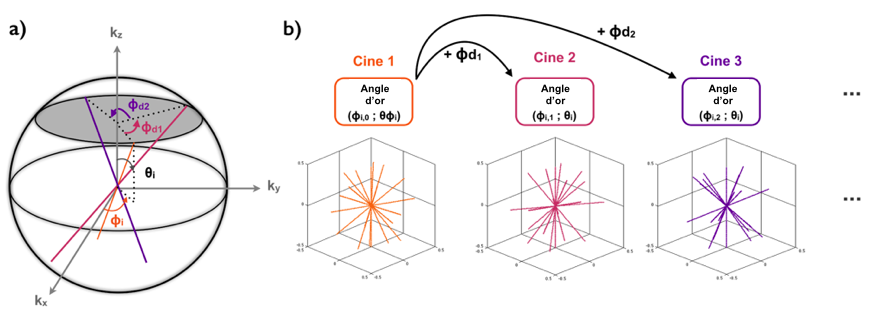
\includegraphics[scale=0.5]{./figure/chap3/GoldCine.png}
\caption[Répartition grâce à l'angle d'or entre les images ciné]{\label{fig:GoldCine} Description de la méthode utilisée pour obtenir une répartition différentes des projections entre des images cinés consécutives. (a) La ligne orange représente la trajectoire d'une projection définie par le premier angle d'or, correspondant à l'image ciné 1 . Pour l'image ciné 2 (rose), la nouvelle trajectoire est obtenue en ajoutant l'angle $\Phi d_1$. Pour l'image ciné 3 (violet), l'angle ajouté est égale à $\Phi d_2$. La même valeur d'angle $\theta_i$, est utilisé entre les projections des cinés adjacentes. (b) Exemple sur la distribution 9 projections pour 3 images cinés consécutives.}
\line(1,0){400} \\ \end{figure}

\begin{figure}[H]
\centering \line(1,0){400} \\
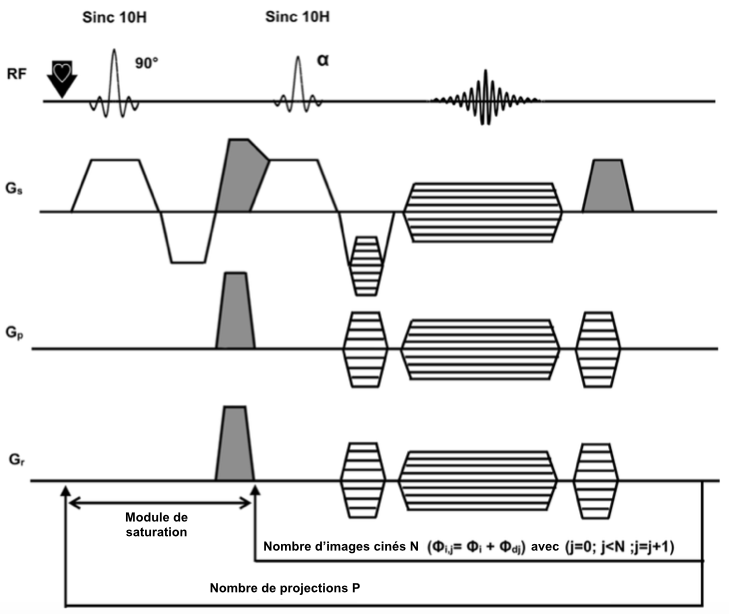
\includegraphics[scale=0.5]{./figure/chap3/SeqARMAurel.png}
\caption[Chronogramme ARM dynamique]{\label{fig:SeqARMAurel} Chronogramme de la séquence ARM sang blanc 3D radiale synchronisé sur l'ECG. Un module de saturation a été ajouté avant l'acquisition de N images cinés. Chacune de ces images a été acquises avec $P(\Phi_{i,j},\theta_i)$ projections. Pour chaque image ciné, $\Phi_{i,j} = \Phi_i+\Phi d_j$, où i est le nombre de projection et j est le nombre de ciné. Les gradients de déphasage sont indiqués en gris. La flèche noire représente la synchronisation ECG.}
\line(1,0){400} \\ \end{figure}

\subsubsection{Méthode de reconstruction flexible}

Pour reconstruire une image ciné à un temps donné du cycle cardiaque, nous avons utilisé un filtre temporel que nous appliquons à chaque espace de Fourier. Ce filtre temporel permet de regrouper les données de l'espace de Fourier que l'on veut reconstruire avec une partie des hautes fréquences des espaces de Fourier adjacents. De nombreux filtres différents peuvent être créés et adaptés a-posteriori lors de la reconstruction comme des filtres exponentielles ou linéaires qui s'utilisent pour des images de prises de contraste dynamique \cite{Lin:2008uq}.
Nous avons décidé d'utiliser un filtre défini par 2 paramètres, Q et R ($Q \leq R$) qui correspondent à des distances temporelles entre les espaces de Fourier dans le cycle cardiaque par rapport à l'espace de Fourier à reconstruire. Pour reconstruire l'image situé à la position x du cycle cardiaque, nous utiliserons tout l'espace de Fourier à cette position auquel nous ajouterons la moitié des hautes fréquences des espaces situé à une position s tel que : $x-Q < s \leq x+Q$ inclus. Et enfin nous ajouterons le quart des hautes fréquences des espaces de Fourier situé à une position $x-Q-R \leq s < x-Q$ et $x+Q \geq s \geq x+Q+R$. La forme de ce filtre est illustré dans la figure \ref{fig:filtre} pour des valeurs R = 3 et Q = 1.
La résolution temporelle est donc étalé sur 7 TR mais le fait de ne pas utiliser les basses fréquences dans les images cinés adjacentes permet de réduire la résolution temporelle effective.
Après application du filtre temporel on obtient un espace de Fourier que l'on peut reconstruire avec la méthode de "gridding" standard décrite dans le chapitre précédente.
L'utilisation d'un filtre temporel n'est pas uniforme sur tout le cycle cardiaque. En effet, des effets de bords réduiront la qualité des images que l'on peut obtenir au début et à la fin du cycle cardiaque.

\begin{figure}[H]
\centering \line(1,0){400} \\
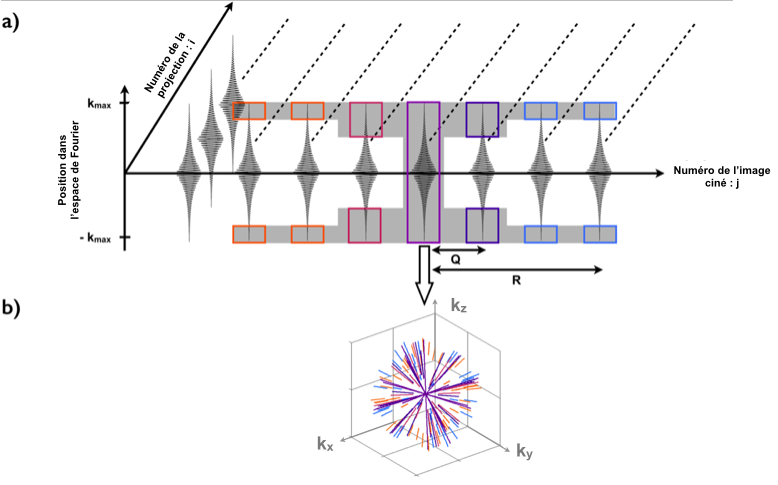
\includegraphics[scale=0.45]{./figure/chap3/filtre.png}
\caption[Filtre temporel]{\label{fig:filtre} Représentation du filtre temporel (en gris) utilisé pour reconstruire l'image ciné 5 avec Q = 1 et R = 3. (a) Les données sont reconstruites en utilisant la moitié des hautes fréquences des projections recueillies à une distance temporelle maximum Q, et un quart des projections est utilisé pour des distances temporelles plus élevées (de Q à R). (b) Représentation schématique de l'espace de Fourier de l'image ciné 5 après application du filtre temporel.}
\line(1,0){400} \\ \end{figure}

\section{Résultat}

\subsection{Système d'imagerie et de gradients}

Les expériences ont été effectuées sur un imageur 7T Bruker Biospec (Ettlingen, Germany) équipé avec un système de gradient capable de fournir 660 mT/m au maximum et avec un temps de monté des gradients de 110 $\mu$s.
Une antenne volumique quadratique (Diamètre interne 75.4 mm, longueur = 70 mm) est utilisée pour l'excitation et une antenne de surface à 4 éléments (dimension extérieur d'un élément d'antenne: 12 $\times$ 16 mm$ ^2$; dimension extérieure totale: 26 $\times$ 21 mm$ ^2$) est utilisée pour la réception du signal.

\subsection{Validation de la séquence}
\subsubsection{In-vitro}
Nous avons tout d'abord déterminer l'effet du sous-échantillonnage et de l'utilisation du filtre temporel sur l'évaluation de la dynamique de progression des flux. Pour cela, nous avons imagé un fantôme constitué de spins stationnaires contenu dans un cylindre remplie avec de l'eau et de spins mouvants dans un tube droit contenant de l'eau. Le diamètre du tube est de 0,5 mm et le débit de l'eau dans le tube est de 3,75 mL/min qui correspond à une vitesse de 31,8 cm/s. La séquence n'est pas synchronisé et 20 images cinés sont recueillies. Nous avons utilisé les paramètres suivant pour l'imagerie: TE/TR = 1,5/3,3 ms; $\alpha=12\degres$; bande passante de réception = 200 kHz; FOV = 25 x 25 x 25 mm; matrice de lecture = 192; résolution spatiale = $(130 \ \mu m)^3$.
\begin{figure}[H]
\centering \line(1,0){400} \\
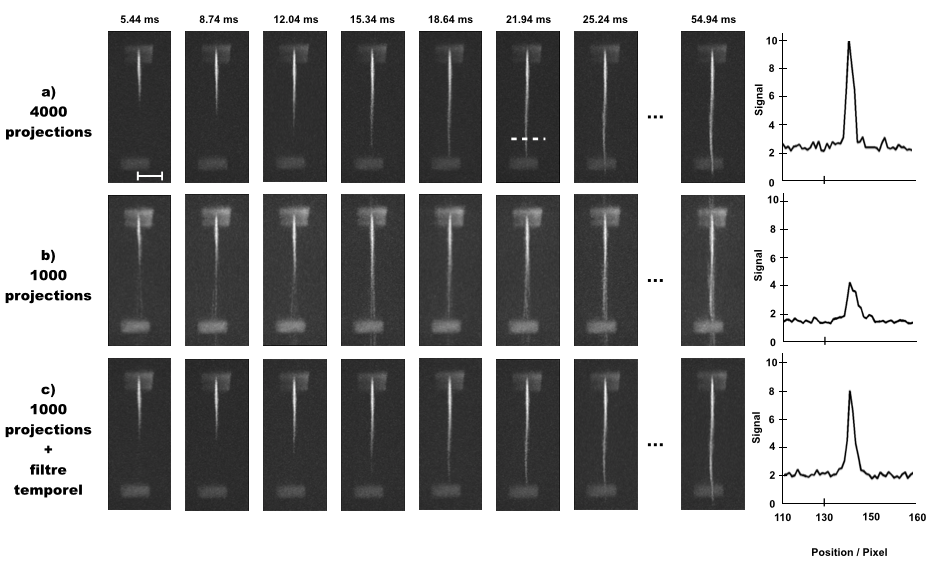
\includegraphics[scale=0.5]{./figure/chap3/ImFlowPhant.png}
\caption[Image ARM dynamique sur fantôme]{\label{fig:ImFlowPhant} Images MIP coronales recueillies sur le fantôme de flux avec la séquence dynamique. Les images reconstruites avec (a) 4000 ou (b) 1000 projections sont comparées aux images reconstruites avec (c) 1000 projections et l'utilisation d'un filtre temporel (R=3, Q=1). Le profile d'intensité est obtenu au niveau de la ligne pointillée au temps 21,94 ms pour chaque cas.}
\line(1,0){400} \\ \end{figure}

Les données sont sous-échantillonnées a-posteriori pour obtenir un jeu de donnée constitué de 1000 et 4000 projections correspondant respectivement à des temps d'acquisition de 4 min 51 s et 1 min 13 s. Avec 4000 projections (figure \ref{fig:ImFlowPhant}.a), nous arrivons a distinctement visualiser la progression du flux dans le tube et sa vitesse peut être correctement mesurée. Le pic de vitesse est égale à 65 cm/s, ce qui correspond à 2 fois la valeur moyenne. Avec 1000 projections (figure \ref{fig:ImFlowPhant}.b), on observe sur les images une nette infériorité en terme de signal et de résolution spatiale. Le signal du tube passe de 10 à 4,2 entre 4000 et 1000 projections. On observe aussi la présence d'artéfacts de streaking (flèche blanche) qui empêche la mesure d'une valeur précise de vitesse des flux. Cependant en utilisant le filtre temporel (R=3,Q=1) (figure \ref{fig:ImFlowPhant}.c) les artéfacts de streaking sont supprimés et l'on observe que le profile de signal remonte de 4.2 à 8 ce qui est environ au niveau de la reconstruction avec 4000 projections.
Nous avons mesuré l'augmentation du volume de flux dans le FOV sur toutes les images ciné (correspondant à la progression du flux dans le tube) et l'on observe une sur-évaluation du volume sur les images reconstruites avec 1000 projections. Par contre avec l'utilisation du filtre on observe des données totalement en accord avec celle reconstruite avec 4000 projections.
\begin{figure}[H]
\centering \line(1,0){400} \\
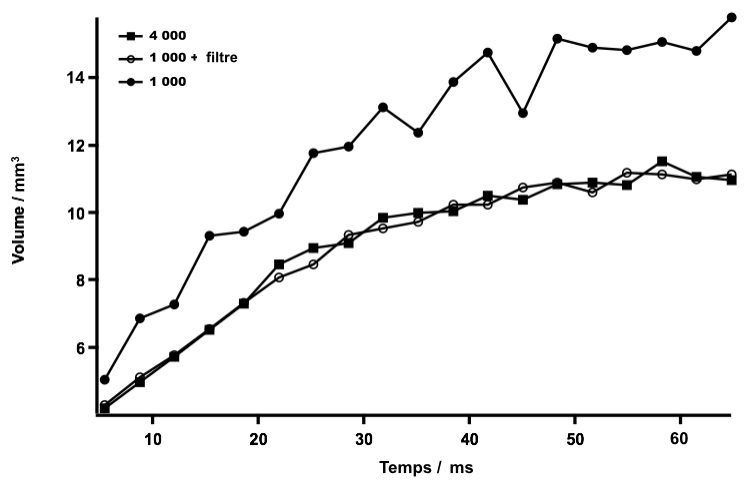
\includegraphics[scale=0.4]{./figure/chap3/GraphFlowPhant.png}
\caption[Graphique de progression du flux sur fantôme]{\label{fig:GraphFlowPhant} Volume des flux mesuré en fonction du temps après l'application du module de saturation obtenues sur fantôme. Les données représentées ont été recueillies avec 4000, 1000 et 1000 + filtre projections.}
\line(1,0){400} \\ \end{figure}

\subsubsection{In-vivo}

Ces observations ont aussi été observé in-vivo sur les carotides de souris avec la même séquence synchronisée sur l'ECG. La comparaison des images non-filtrée et filtrée avec 1000, 2500 et 4000 projections (figure \ref{fig:ImFlowMice}) ainsi que les résultats de mesure de volume de flux (\ref{fig:GraphFlowMice}) montre qu'il est nécessaire d'utiliser un nombre de projection plus important in-vivo due à la qualité globale des images. Les images obtenue avec une reconstruction de 2500 projections et l'utilisation du filtre (R=3,Q=1) donne des résultats équivalent en terme de qualité d'image et de volume du flux. Dans la suite, nous utiliserons 2500 projections correspondant approximativement à 6 min 30 s de temps d'acquisition totale.
\begin{figure}[H]
\centering \line(1,0){400} \\
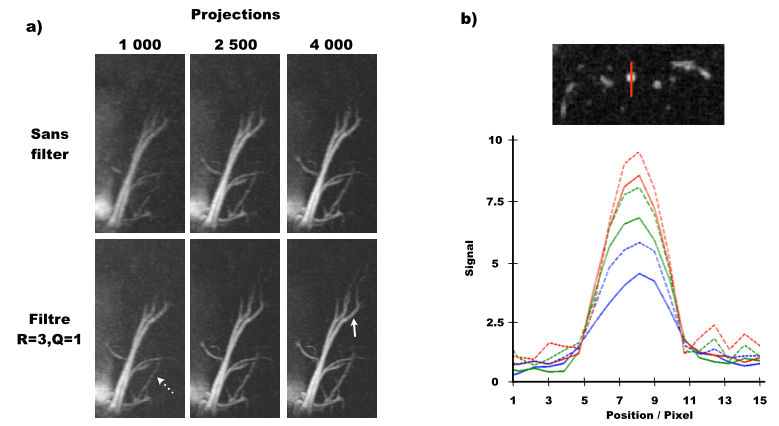
\includegraphics[scale=0.5]{./figure/chap3/ImFlowMice.png}
\caption[Image ARM dynamique sur souris]{\label{fig:ImFlowMice} Images MIP sagital recueillies sur des carotides de souris avec la séquence dynamique. (a) Les images reconstruites avec 1000, 2500 et 4000 projections sont comparées aux images reconstruites avec l'utilisation d'un filtre temporel (R=3, Q=1). (b) Le profile d'intensité est obtenu au niveau de la ligne rouge sur les carotides après la bifurcation aortique. Lignes continues : reconstructions non-filtrées; bleu: 1000 projections; vert: 2500 projection; rouge: 4000 projections.}
\line(1,0){400} \\ \end{figure}

\begin{figure}[H]
\centering \line(1,0){400} \\
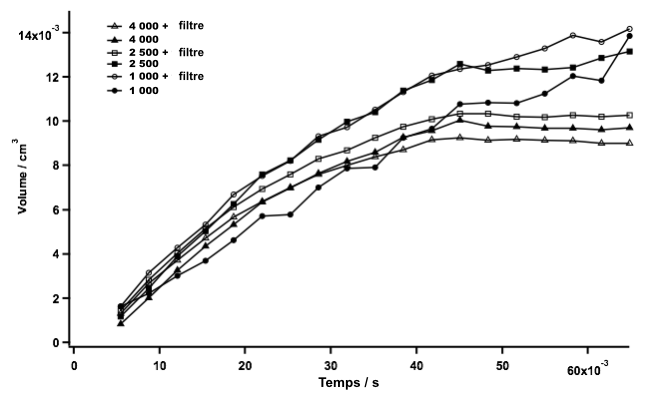
\includegraphics[scale=0.5]{./figure/chap3/GraphFlowMice.png}
\caption[Graphique de progression du flux sur fantôme]{\label{fig:GraphFlowMice} Volume des flux mesuré en fonction du temps après l'application du module de saturation sur les carotides d'une souris saine. Les données représentées ont été recueillies avec 4000, 2500 et 1000 projections ainsi qu'avec leurs reconstruction filtrée (R=3,Q=1).}
\line(1,0){400} \\ \end{figure}

\subsection{Imagerie du polygone de Willis}

Avec la séquence d'ARM dynamique, il a été possible de visualiser chez 4 souris ayant subit une ligature de la carotide droite que le remplissage du polygone était compensé par le flux sanguin provenant de la carotide droite. Cependant celui-ci arrive dans la partie droite du polygone avec un délai de retard par rapport à la souris saine (\ref{fig:ImFlowWillis}).
Ce délai a pu être quantifier sur une carte de couleur grâce à une méthode de calcule du temps d'arriver du sang en un point de l'espace (\ref{fig:ColorMapFlowWillis}).

\begin{figure}[H]
\centering \line(1,0){400} \\
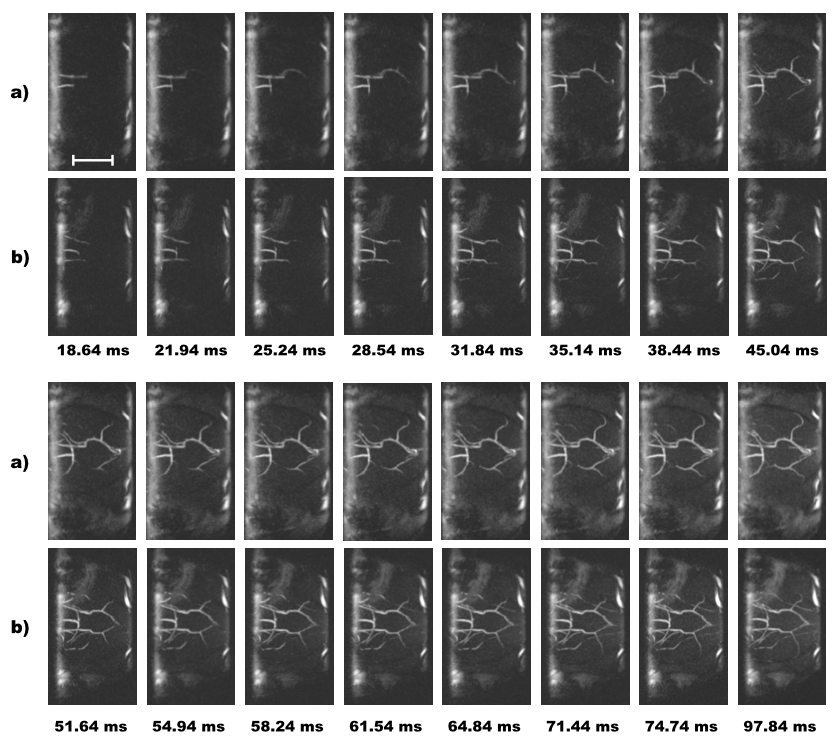
\includegraphics[scale=0.5]{./figure/chap3/ImFlowWillis.png}
\caption[Image d'ARM dynamique sur souris du polygone de Willis]{\label{fig:ImFlowWillis} Image MIP d'ARM dynamique acquises sur une souris saine (a) et pour une souris ayant subit une ligature des artères carotides (b). 16 images ont été extraites des 30 images cinés acquises.}
\line(1,0){400} \\ \end{figure}

\begin{figure}[H]
\centering \line(1,0){400} \\
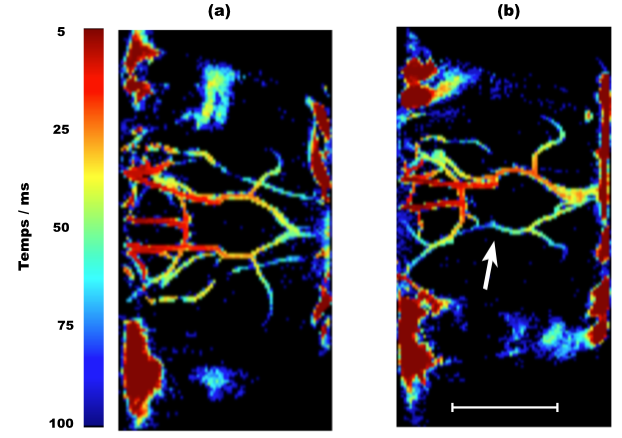
\includegraphics[scale=0.5]{./figure/chap3/ColorMapFlowWillis.png}
\caption[Image d'ARM dynamique sur souris du polygone de Willis]{\label{fig:ColorMapFlowWillis} Carte de couleur représentant la durée avant l'arrivée du sang dans une partie du polygone de Willis pour une souris saine (a) et une souris avec une artère carotide ligaturée (b).}
\line(1,0){400} \\ \end{figure}

Il n'est pas possible d'effectuer l'imagerie sur une plus large zone (par example des carotides au polygone). En effet, le contraste étant basé sur le principe du temps de vol, celui-ci sera saturé en arrivant à la fin du polygone. Une des solutions est d'augmenter le TR de la séquence mais nous obtiendrons une moins bonne visualisation dynamique de l'avancée du flux. De plus, la différence entre deux images consécutives sera plus importante ce qui limitera la taille du filtre temporel que l'on pourra utiliser. Enfin un dernier problème se pose puisqu'il faudrait augmenter le nombre d'images cinés à lire après la saturation du signal et donc que le signal statique aura repousser suffisamment pour encore diminuer le contraste que l'on pourrait espérer obtenir entre le cerveaux et les vaisseaux.

L'alternative que nous avons employé est d'appliquer la séquence 3 fois de suite en modifiant la position de la coupe puis à associer les images après la reconstruction en fonction de leurs positions (figure \ref{fig:FluxComplet}.a). On peut aussi reconstruire une carte de couleur mais cela demande à l'utilisateur d'indiquer à quel moment le flux d'une coupe entre dans la suivante. La figure \ref{fig:FluxComplet}.b est un example de représentation en carte de couleur utilisant de multiples coupes. On observe sur ces images des artéfacts au bord des coupes qui sont due à la mauvaise saturation du signal au bord de la sélection de coupe.

\begin{figure}[H]
\centering \line(1,0){400} \\
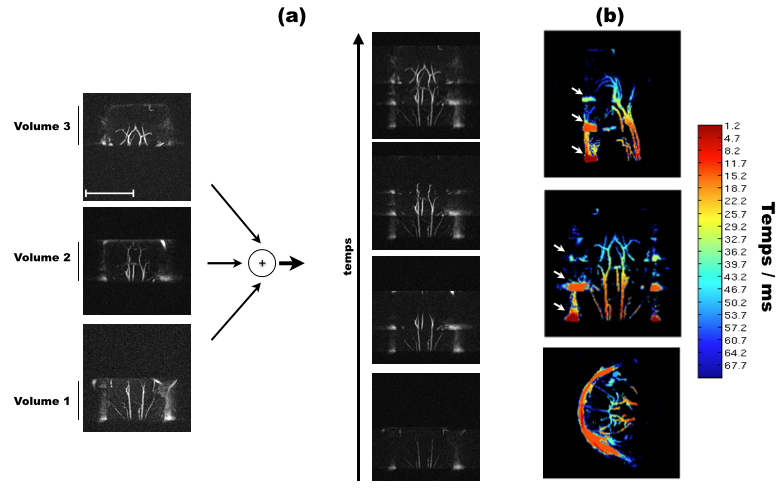
\includegraphics[scale=0.6]{./figure/chap3/FluxComplet.png}
\caption[Image d'ARM dynamique sur souris des carotides au polygone de Willis]{\label{fig:FluxComplet} Imagerie des carotides au polygone effectuée avec 3 acquisitions successives avec des coupes en 3 positions différentes. (a) L'association des images est effectuées après la reconstruction de chacune d'entre elles. (b) La carte de couleur représentant l'avancée des flux doit être synchronisé pour que l'arrivée d'une du sang dans la prochaine coupe débutent en même temps que le début de la prochaine.}
\line(1,0){400} \\ \end{figure}

\section{Discussion}

L'imagerie de flux chez la souris est un véritable défi du fait de la dimension des vaisseaux des paramètres physiologiques particuliers de la souris. De telles méthodes permettraient de mieux décrire le phénotype des modèles et suivre l'évolution des pathologies lors d'études longitudinales. Le développement de nouvelles méthodes d'imageries 4D de flux dynamique, offrant une résolution spatiale et temporelle élevée durant un temps d'acquisition raisonnable sont nécessaires pour accéder avec précision aux données fonctionnelles des flux.

Dans cette optique nous avons tout d'abord développé une séquence avec une trajectoire 3D radiale (PR) pour l'ARM anatomique. En effet, cette méthode est peu sensible aux artéfacts de flux et de mouvements que l'imagerie cartésienne ce qui permet d'obtenir des images anatomiques de la crosse aortique avec un signal très homogène malgré la respiration et les flux turbulent durant la phase systolique du coeur. De plus, la possibilité de sous-échantillonnage de cette méthode nous a permis d'obtenir des images ayant une qualité satisfaisante avec seulement 4000 projections correspondant à une diminution du temps d'acquisition supérieur 10 par rapport au critère de Nyquist. Le troisième avantage de l'imagerie radiale est l'utilisation d'une trajectoire de type angle d'or. Cela permet une distribution approximativement uniforme des projections au cours du temps même. Cette méthode peut être employé pour efficacement répartir les projections avec pour objectif de retirer les projections corrompues par les mouvements physiologiques.

Nous avons ensuite étendu cette approche à l'imagerie résolue dans le temps pour visualiser la progression des flux dans les vaisseaux avec une très forte résolution temporelle tout en maintenant un temps d'acquisition limité. Nos résultats ont montré

%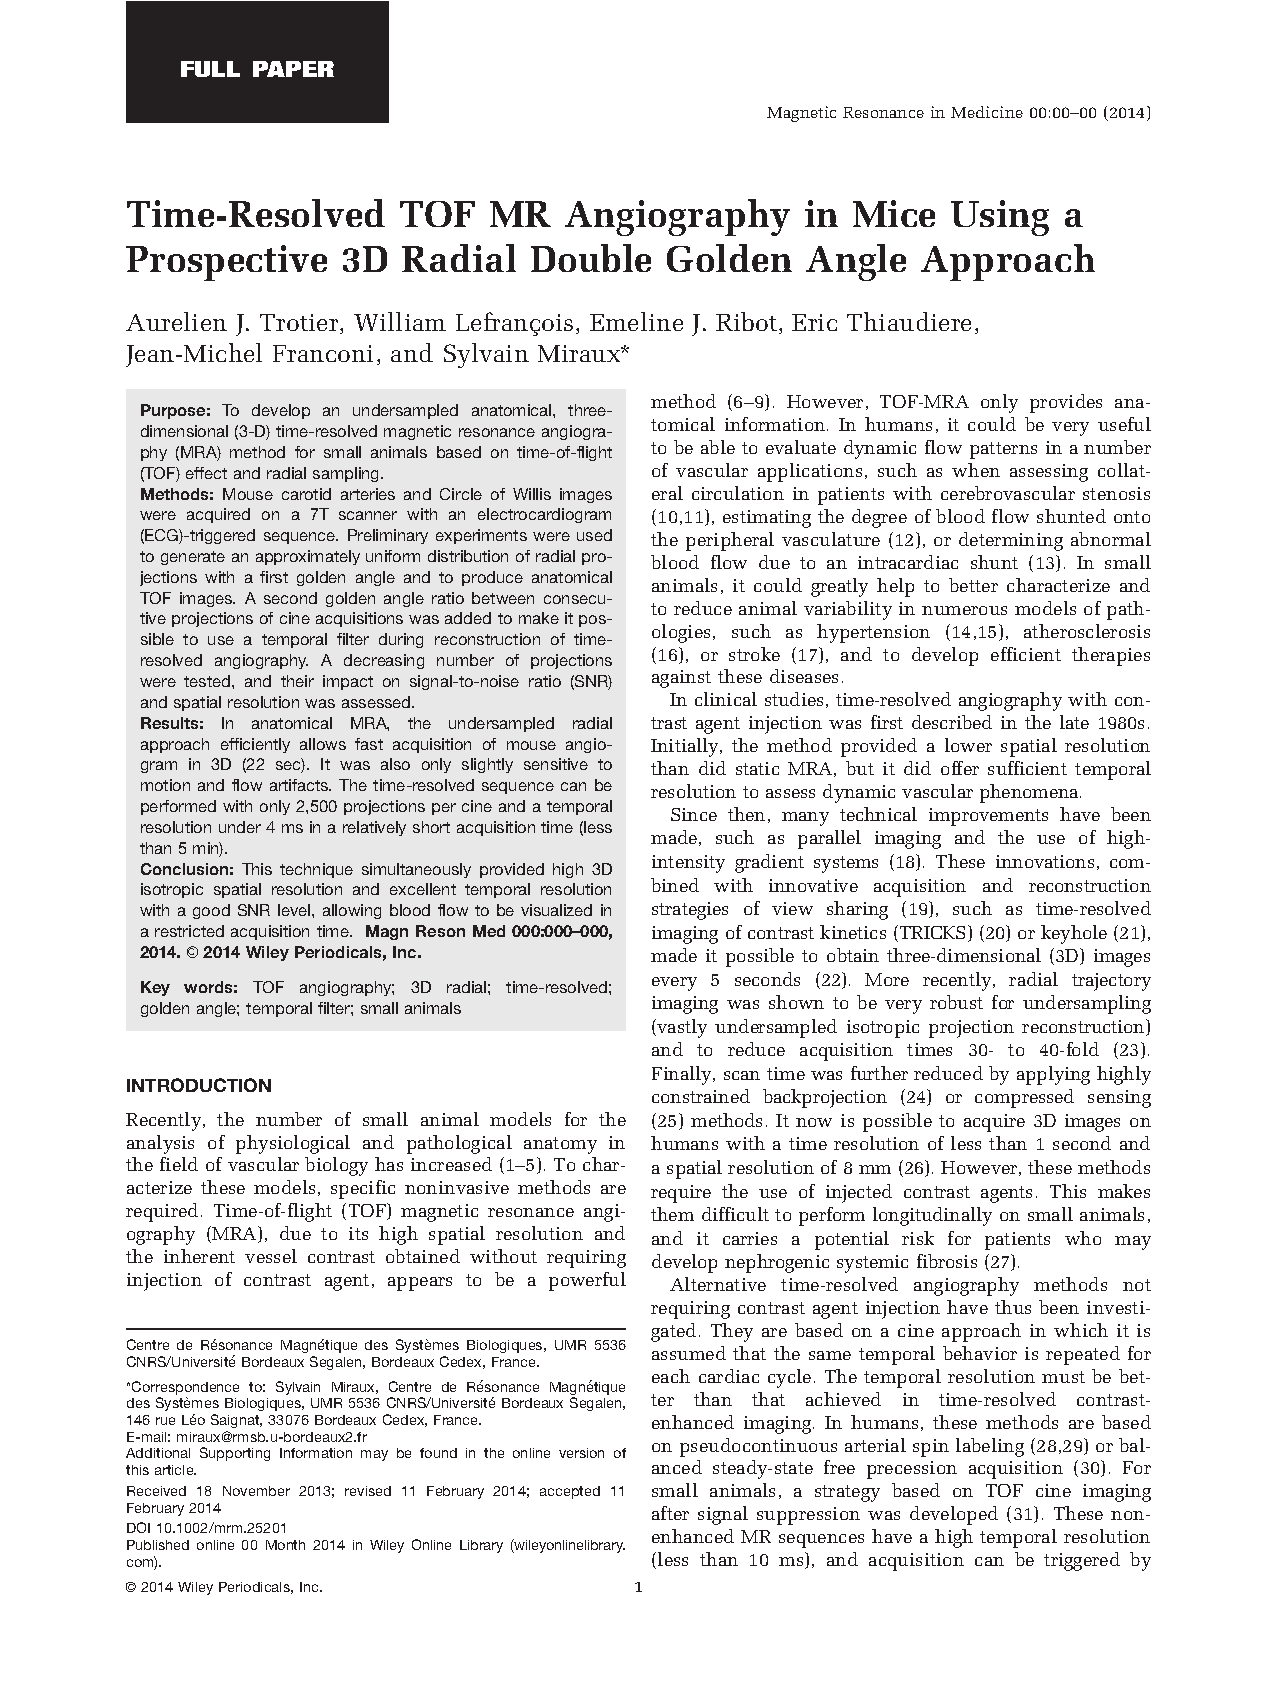
\includepdf[pages=1-11]{./figure/chap3/Papier1.pdf}